\usetikzlibrary{arrows.meta,shapes.symbols}
\begin{frame}{conections}
    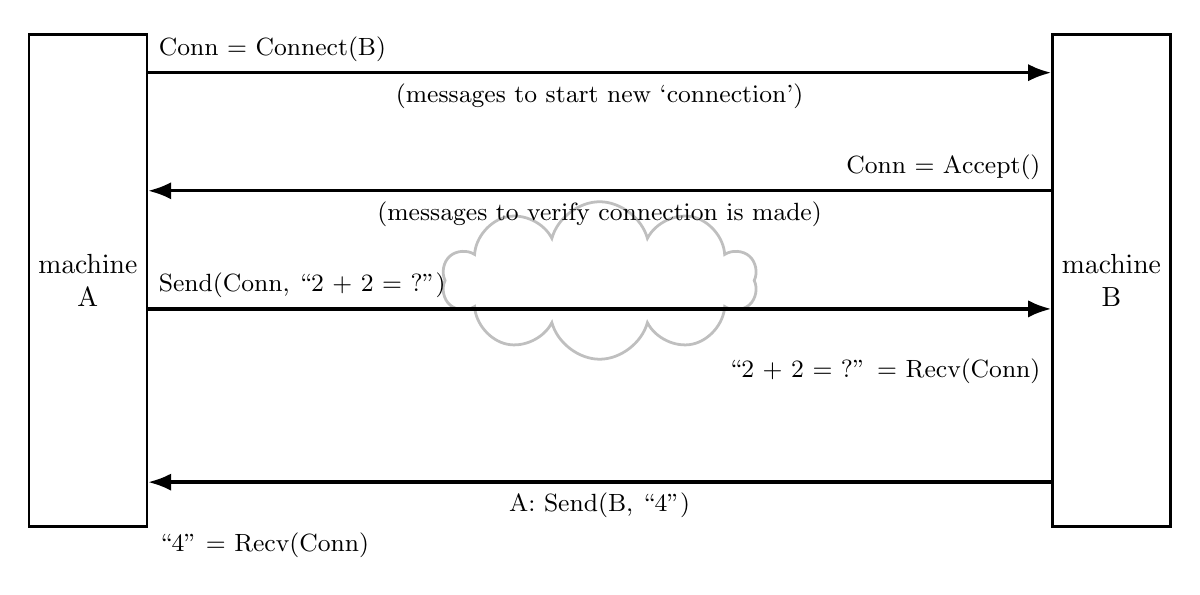
\begin{tikzpicture}
    \tikzset{
        >=Latex,
        comp box/.style={draw, thick, align=center, minimum width=1.5cm,minimum height=6.25cm},
        explain box/.style={draw=red,very thick, align=left},
        msg/.style={font=\small},
        cmd/.style={font=\small},
    }
        \node[comp box] (machine A) at (-6.5, 0) {machine \\ A};
        \node[draw,cloud,line width=1pt,minimum width=4cm,minimum height=2cm,aspect=3,opacity=0.25] (network) at (0,0) {~~};
        \node[comp box] (machine B) at (6.5, 0) {machine \\ B};
        \draw[very thick,->] ([yshift=-.5cm]machine A.north east) -- ([yshift=-.5cm]machine B.north west) 
            node[midway,below,msg] {(messages to start new `connection')}
            node[pos=0.0,above right,cmd] {Conn = Connect(B)};
        \draw[very thick,<-] ([yshift=-2cm]machine A.north east) -- ([yshift=-2cm]machine B.north west) 
            node[midway,below,msg] {(messages to verify connection is made)}
            node[pos=1.0,above left,cmd] {Conn = Accept()};
        \draw[very thick,->] ([yshift=-3.5cm]machine A.north east) -- ([yshift=-3.5cm]machine B.north west) 
            %node[midway,below,msg] {B: Send(A, ``2 + 2 = ?'')}
            node[pos=0.0,above right,cmd] {Send(Conn, ``2 + 2 = ?'')}
            node[pos=1.0,below left,cmd,yshift=-.5cm] {``2 + 2 = ?'' = Recv(Conn)};
        \draw[very thick,<-] ([yshift=-5.7cm]machine A.north east) -- ([yshift=-5.7cm]machine B.north west) 
            node[midway,below,msg] {A: Send(B, ``4'')}
            %node[pos=1.0,above left,cmd] {Send(Conn, ``4'')}
            node[pos=0.0,below right,cmd,yshift=-.5cm] {``4'' = Recv(Conn)};
    \end{tikzpicture}
\end{frame}

